\begin{frame}{SmartFin}
    \begin{columns}[c] % The 'c' option vertically centers the content in the columns
        \begin{column}{0.5\textwidth}
            \centering
            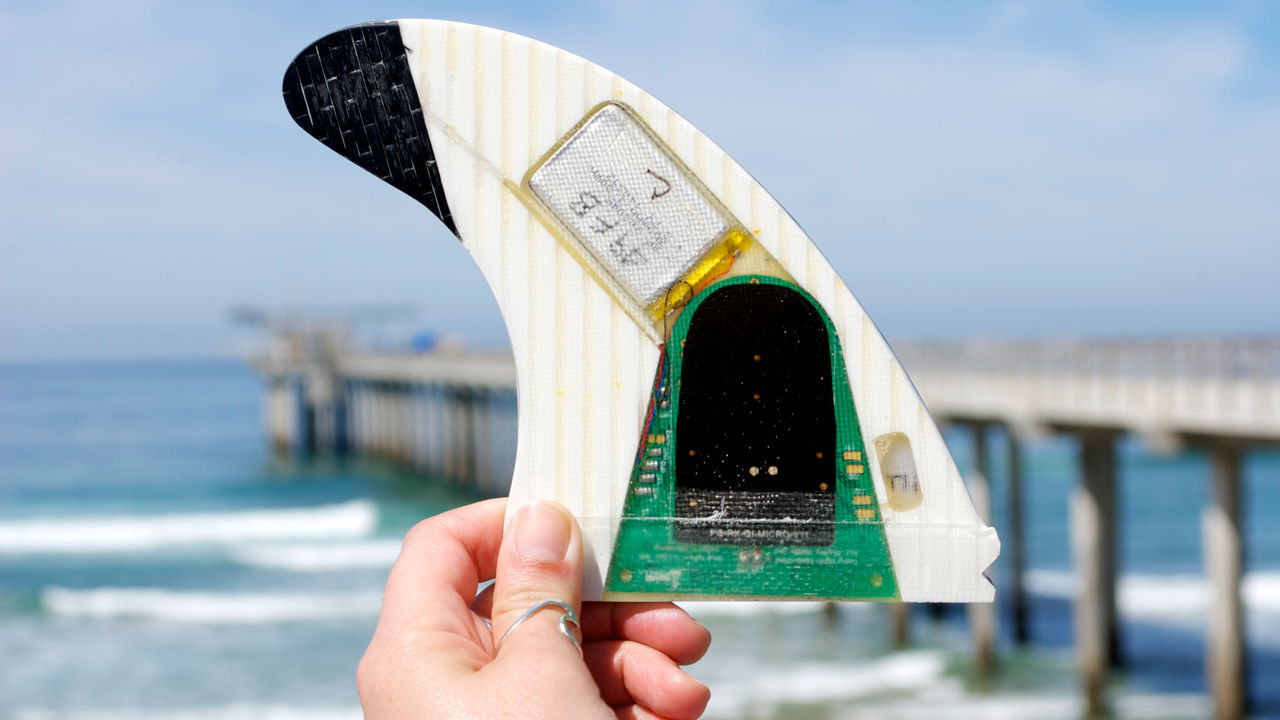
\includegraphics[width=0.9\linewidth]{images/smartfin_picture.jpg}
        \end{column}
        \begin{column}{0.5\textwidth}
            \justifying % Justifies the text in this column
            Smartfin is an oceanographic sensor-equipped surfboard fin used by surfers and paddlers in surf zone and nearshore regions.
        \end{column}
    \end{columns}
\end{frame}
\begin{frame}{Why Not Buoys?}
    \begin{columns}[c]
        \begin{column}{0.5\textwidth}
            \centering
            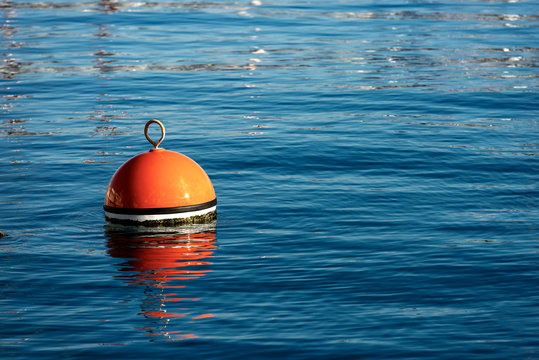
\includegraphics[width=0.9\linewidth]{images/buoy.jpg}
            \vspace{0.5em}
            {\small Buoys are key tools for ocean and climate data.}
        \end{column}
        \begin{column}{0.5\textwidth}
            \centering
            \includegraphics[width=0.9\linewidth]{images/surfzone.gif}
            \vspace{0.5em}
            {\small Surf zones are too crowded and dynamic for traditional buoys.}
        \end{column}
    \end{columns}
    \vspace{1em}
    \begin{center}
    \textbf{Smartfin allows surfers to collect critical nearshore data.}
    \end{center}
\end{frame}
\begin{frame}{How Far Along Are We?}
    \begin{center}
        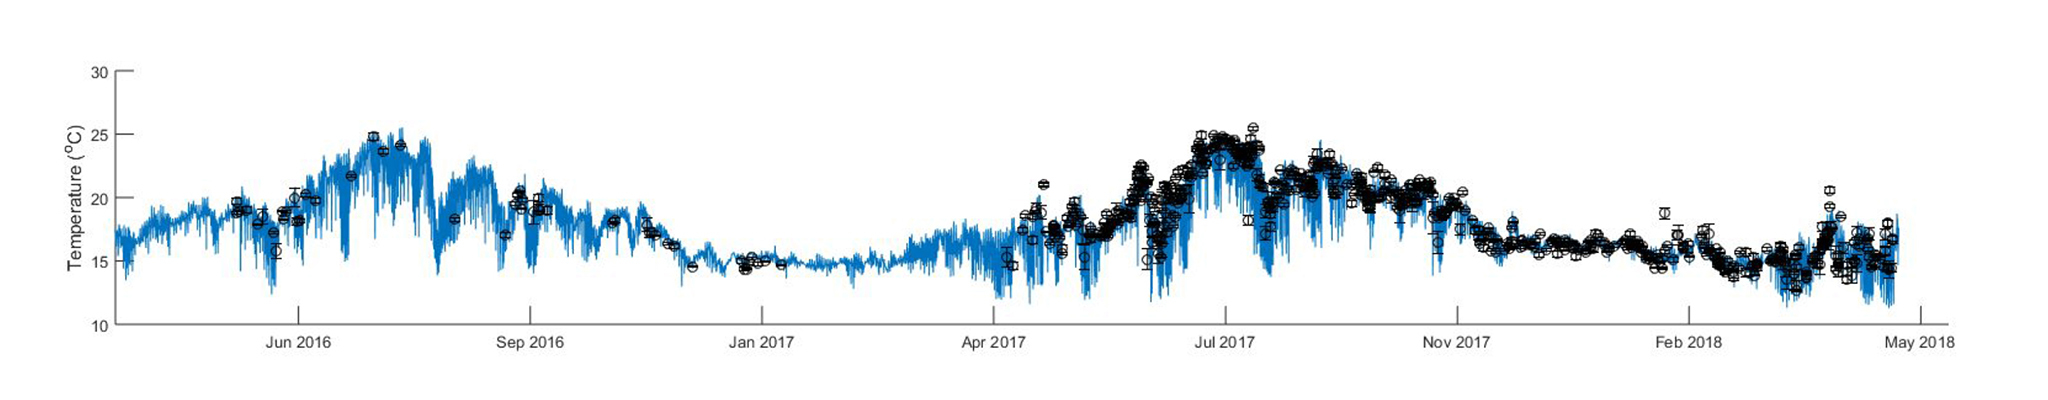
\includegraphics[width=0.7\textwidth]{images/buoy_vs_smartfin_data.jpg}
        \vspace{1em}
        \small Smartfin data aligns closely with buoy measurements. 300+ Smartfins deployed globally.
    \end{center}
\end{frame}
\begin{frame}{My Goals for the Summer}
    \begin{columns}[c]
        \begin{column}{0.45\textwidth}
            \centering
            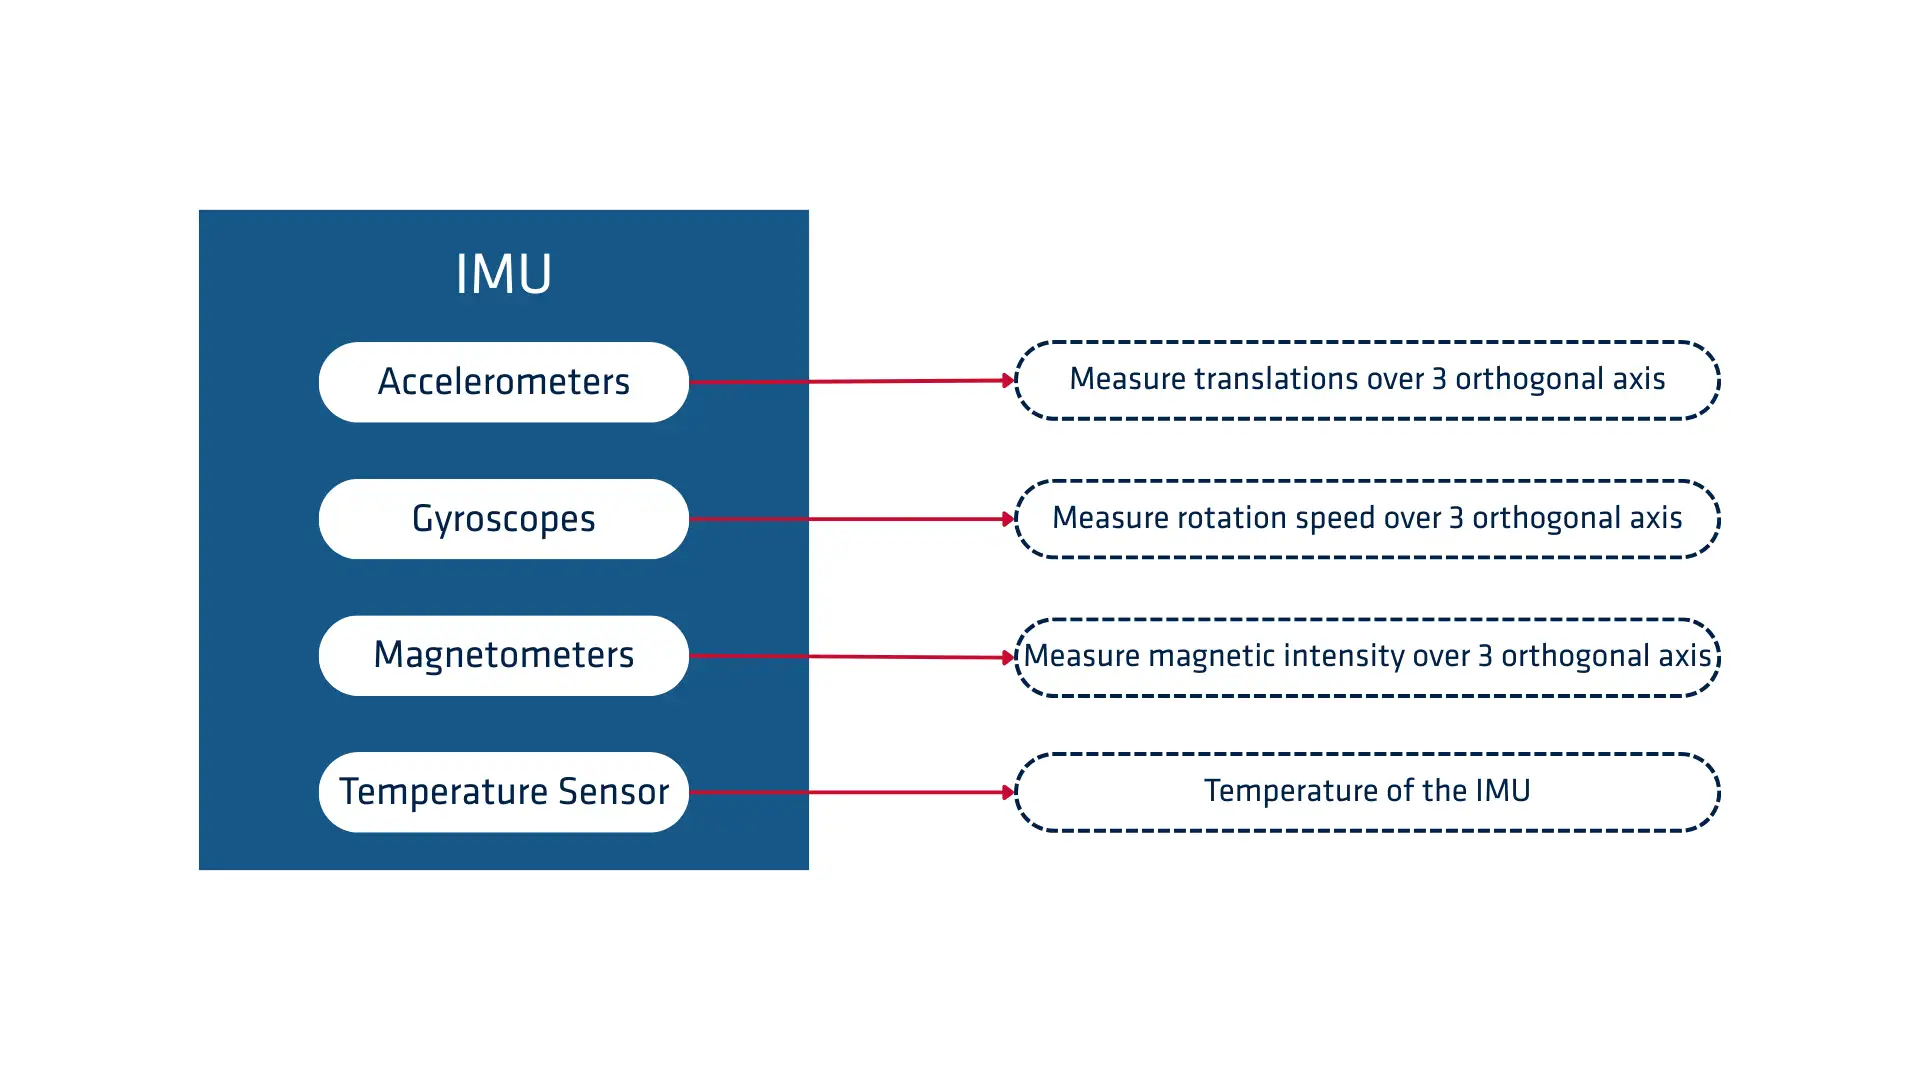
\includegraphics[width=0.85\linewidth]{images/imu-diagram.png}
        \end{column}
        \begin{column}{0.55\textwidth}
            \small
            \textbf{Key Variables to Analyze:}
            \begin{itemize}
                \item \textbf{Temperature:} Accuracy, Precision, Rise/Fall Time
                \item Wet/Dry Threshold
                \item \textbf{GPS:} Change of Position/Time
                \item \textbf{Accelerometer:} Accuracy, Precision, Orthogonality
                \item Gyroscope, Magnetometer
            \end{itemize}
            IMU data helps calculate attitude, angular rates, and motion relative to Earth.
        \end{column}
    \end{columns}
\end{frame}
\begin{frame}{Plan for the Next Week}
    \begin{columns}[T]
        \begin{column}{0.5\textwidth}
            \centering
            \includegraphics[width=0.9\linewidth]{images/sst_chart.png}
        \end{column}
        \begin{column}{0.5\textwidth}
            \centering
            \includegraphics[width=0.9\linewidth]{images/static_test_chart.png}
        \end{column}
    \end{columns}
    \vspace{1em}
    \begin{center}
        \small Sensor validation using SST accuracy and static IMU tests in controlled environments.
    \end{center}
\end{frame}